% Teste de uma tabela:

% \begin{table}[htb]
% 	% Título de tabelas sempre aparecem antes da tabela
% 	\textsf{\caption{Tabela sem sentido}}
% 	\center
% 	{
% 		\begin{tabular}{l|l}
% 			\hline
% 			Titulo Coluna 1   & Título Coluna 2\\
% 			\hline
% 			X                 & Y\\
% 			X                 & W\\
% 			\hline
% 		\end{tabular}
% 	}
% 	\label{tab:TabelaSemSentido}
% \end{table}
% 
% $Referência à tabela definida no início: \ref{tab:TabelaSemSentido}

% \begin{figure}[htb]
% 	\centering
%   	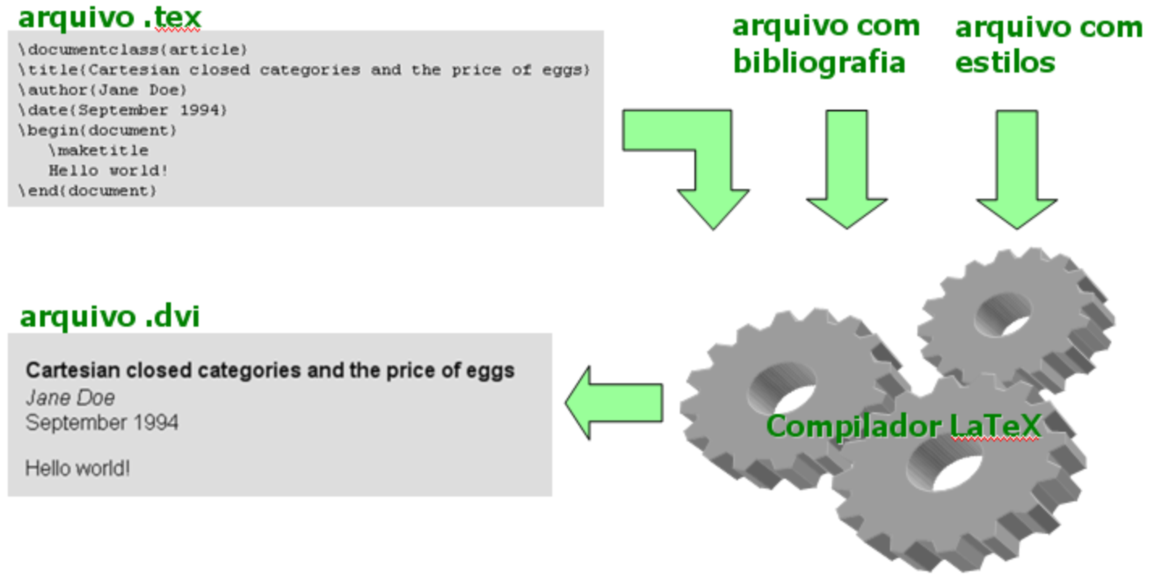
\includegraphics[scale=7.0]{Imagens/FiguraTeste.png}
%   	\textsf{\caption{Teste de uma figura em formato .png}}
%   	\label{fig:FiguraTeste}
% \end{figure}

% Referenciamento da figura inserida na seção anterior: \ref{fig:FiguraTeste}

% \simb[$\lambda$ (algum símbolo)]{$\lambda$}

% \abrv[UFRN -- Universidade Federal do Rio Grande do Norte]{UFRN}

% \cite{siri} é um programa.
% 
% Na tese de Doutorado de Paquete \cite{PaquetePhD}, discute-se sobre algoritmos de busca local estocásticos aplicados a problemas de Otimização Combinatória considerando múltiplos objetivos. Por sua vez, o trabalho de \cite{KnowlesBoundedLebesgue}, publicado nos anais do IEEE CEC de 2003, mostra uma técnica de arquivamento também empregada no desenvolvimento de algoritmos evolucionários multi-objetivo, trabalho esse posteriormente estendido para um capítulo de livro dos mesmos autores \cite{KnowlesBoundedPareto}. Por fim, no relatório técnico de \citeonline{Jaszkiewicz}, fala-se sobre um algoritmo genético híbrido para problemas multi-critério, enquanto no artigo de jornal de Lopez \textit{et al.} \cite{LopezPaqueteStu} trata-se do \textit{trade-off} entre algoritmos genéticos e metodologias de busca local, também aplicados no contexto multi-critério e relacionado de alguma forma ao trabalho de Jaszkiewicz (\citeyear{Jaszkiewicz}).
% 
% Outros exemplos relacionados encontram-se em \cite{Silberschatz} (livro), \cite{DB2XML} (referência da Web) e \cite{Angelo} (dissertação de Mestrado).